\section{Dégagement des contraintes de développement}

Selon des fonctions définies et des codes existantes, j'ai défini des contraintes et proposé des solutions :


\subsection{La gestion d'utilisateurs}

\textbf{Contraintes} 

\begin{itemize}
    \item Manque d'un système d'accès connecté celui de l’écoles
    \item Sans reconnaissance d’identités
\end{itemize}

J'ai proposé :

\begin{itemize}
    \item Communiquer avec les responsables informatiques d'écoles pour intérroger des méthodes de connection
    \item Réaliser la reconnaissance selon les mails address \footnote{ Par exemple, @eleves.ec-nantes.fr indique un élève et @ec-nantes.fr indque un enseignant } 
    \item Avant l'intégration de comptes, un système d'autorisation provisoire ressemblant celui d'ezb sera réalisé
    \item Des messageries à ajouter supplémentairement à la fin
\end{itemize}


\subsection{La gestion de livre}

\textbf{Contraintes} est :Manque de possibilités d'utilisation de multi-format et téléchargement.

J'ai proposé :

\begin{itemize}
    \item Sauvegarder des fichiers en format XML, TEI précisement, pour sa utilisation générale dans le domaine de livre numérique
    \item Chercher des outils de transformations, sinon il faut fabriquer un 
    \item Permettre le créateur d'un livre de définir son status, publique ou privé, pour éviter des problèmes de copyright
\end{itemize}


\subsection{La gestion de groupes}

\textbf{Contraintes} :Trop de niveaux à choisir quand ajouter un membre qui comprend même le niveau Créateur.

J'ai proposé :Ajouter des membres sans définir leur rôle, ne choisir qu'un seul membre comme le manager du groupe.


\subsection{La gestion de projets}

\textbf{Contraintes}

\begin{itemize}
    \item Impossibilité de définir la finalité par utilisateurs et de les distribuer aux sous-groupes
    \item Difficulté d'organiser des citations, résumés, écritures créatives, etc dans un layer
    \item Manque des contrôles de layers et des possibilité d'inviter des autres éditeurs hors du groupe
\end{itemize}

La nouvelle conception de l'application peut être présentée dans trois parties principales, la structure de projets, la distribution de projets et la contribution de projets.

\begin{figure}[H]
\centering
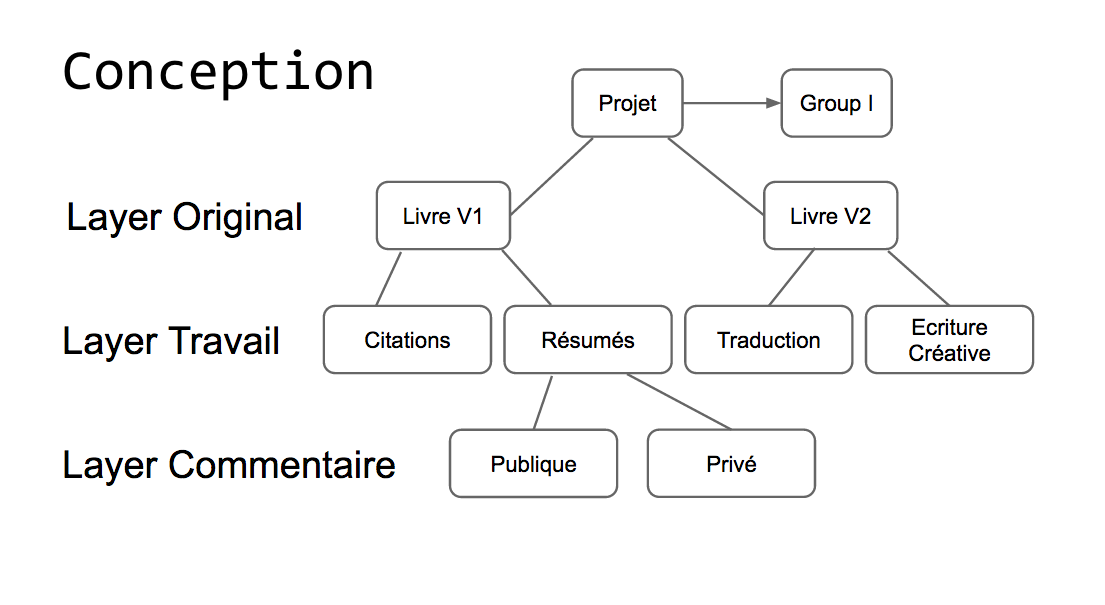
\includegraphics[width=\textwidth]{conception1}
\caption{Structure de projets}
\end{figure}

\begin{figure}[H]
\centering
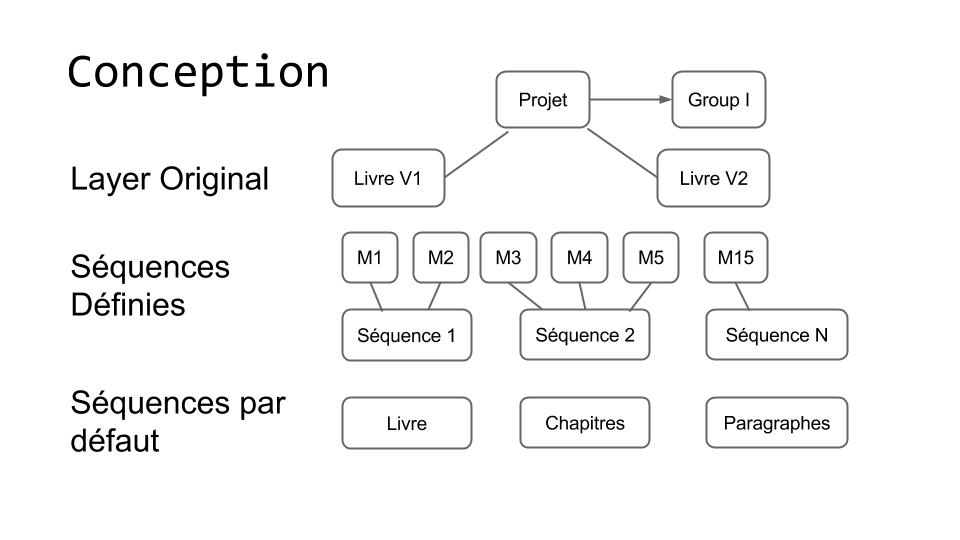
\includegraphics[width=\textwidth]{conception2}
\caption{Distribution de layers}
\end{figure}

\subsubsection{La structure de projets}
Pour garder la flexibilité de multi-échelles et la possibilité de création de layers contenant des citations et autres écritures, j'ai proposé un compromis :

\begin{itemize}
    \item Possible de choisir Privé comme le status d'un layer qui sera invisible pour le publique ni copi-able
    \item Livres sont traités comme layers originals où et on peut définir des marqueurs et des séquences dessus
    \item Il y a deux types de layer travail :
        \begin{itemize}
            \item layer travail \textbf{non-structuré} qui n'est fondé que sur un layer original
            \item layer travail \textbf{structuré} qui est fondé sur un layer original ou un layer travail non-structuré ou structuré
        \end{itemize}
    \item Layers commentaires n'ont pas de sous-layer, ils sont invisible pour le publique ni copi-able et leur status représente la visibilité pour des autres membres de groupe exlclus des éditeurs atorisés.
\end{itemize}

Cette structure permettent d'une création de layer multi-échelles,

\subsubsection{La distribution de projets}
Un autre problème des deux conceptions existantes est de ne pas pouvoir couper un livre dans plusieurs morceaux et les distributer aux sous-groupes d'élèves selon l'esprits d'enseignants. En même temps, il faut fournir des choix de finalités raisonnables automatiquement pour éviter trop de travail. Selon les contraintes, j'ai proposé :

\begin{itemize}
    \item Introduire les conception \textbf{Marqueur}, qui indique une position dans le livre, et \textbf{Séquence}, qui permet de choisir un marqueur au début, un à la fin et des élèves d'édition
    \item Permettre de choisir la finalité comprenant celle définie par utilisateur, mais aussi d'entier livre ou de chapitres ou de paragraphes fournies automatiquement par la plate-forme, pour chaque layer travail pour réaliser différent type d'écriture \footnote{ Par exemple, utiliser la finalité de paragraphes pour la traduction, utiliser la finalité de chapitres pour les résumés de chapitres, etc...} 
    \item Si les élèves travaillent dans un layer distribué de la manière définie par enseignants, ils ne peuvent éditer que dans la séquences autorisée.
\end{itemize}

\subsubsection{La contribution de projets}

\begin{itemize}
    \item \textbf{Layers travail non-structuré} sont vides quand créés, ils supportent deux types d'ajouts :des citations et des écritures libres \footnote{ traduction, résumés, écritures créatives, ect... }
    \item \textbf{Layers travail structuré} qui correspond automatiquement aux travails dans le layer parent, ils ne soutient que les écritures libres correspondants le même morceau de travail de son parent layer
    \item \textbf{Layers commentaires} ont la même structure de son layer parent à commenter, et leurs visibilités sont définies par leurs status.
    \item L'édition est réalisée de la manière synchronisée, tous les travails sont visibles pendant l'édition.
\end{itemize}

En bref, 

\begin{itemize}
    \item \textbf{Layers originals} représentant des livres sont des bases de projets
    \item \textbf{Layers travail} garantissent une structure multi-échelles, mais avec la contrainte de ne pas pouvoir faire des citations hors layers originals
    \item \textbf{layers commentaires} sont les dernières feuilles des braches
    \item D'ailleurs, la nouvelle conception de projets permet d'inviter des autres personnes pour contribuer dans le projet ou commenter des travails faits par des élèves. 
\end{itemize}